
\subsection{Gathering statistical data}
\label{ssub:statisticaldata}
In addition to storing data about each occupant we also store data about how occupied each section of the recorded image is. The process is simple; we split the image of a room into sections, referred to as cells, and each time an occupant enters a cell the stored activity for the given cell is increased. Each room has a different and independent set of cells. This data tells us which sections of the room are most occupied. We use the activity data to perform predictions about an occupant's future actions using a custom prediction model.

\subsection{Custom prediction model based on HMM}
\label{ssub:designcustomprediction}
We have chosen to build our own prediction model heavily inspired by the hidden Markov model. Each cell in the image is a state where the state transition probability is the likelihood of an occupant moving to an adjacent cell and the output probability is the likelihood of an occupant going to an exit given any current cell. Unlike a regular hidden Markov model, we do not store probability values individually for each state, but rather do the necessary calculations each time a prediction is requested by using the stored activity values of each cell. Additionally, our custom model allows us to take several custom factors into account during calculations. These factors work as a rule set for likely or unlikely occupant actions:
\begin{itemize}
\item An occupant entering a room from a given exit is less likely to exit the room at the given exit.
\item An occupant is more likely to continue moving in his general direction and least likely to return to his previously visited cell.
\item An occupant is more likely to move to the adjacent cell with the highest amount of previous activity.
\item The likelihood of an occupant exiting at a given exit (unless it also serves as the occupant's entrance) is inversely proportional to the direct distance to the given exit, producing a magnet-like effect. 
\end{itemize}
These factors have an influence on a final value of a cell or exit, which is used when calculating each probability. The sum of the probabilities of an occupant moving to each individual exit given a current cell is 100. The cell with the highest probability will be the predicted cell.
\begin{figure}[ht]
\centering
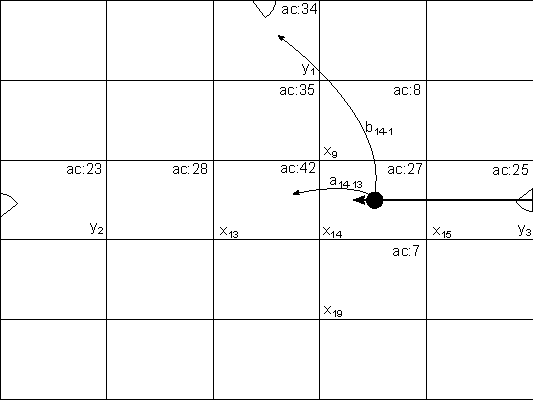
\includegraphics{prediction_figures/custom}
\caption{Applying the custom model to a scenario.}
\label{fig:custom_model}
\end{figure}

Figure \ref{fig:custom_model} shows the custom model translated to a scenario. Each cell contains an identification number, an activity count and a value denoting whether or not the cell is an exit cell. The occupant entered the room at exit \(y_3\) and the current state is \(x_{14}\). \(a_{14-13}\) denotes the state transition probability of the occupant moving from state \(x_{14}\) to state \(x_{13}\). \(b_{14-1}\) denotes the output probability of the occupant ultimately choosing exit \(y_{1}\). Taking our custom rule set into account, the occupant is least likely to exit at \(y_3\) and most likely to continue to \(x_{13}\). Moving to \(x_9\) would increase the probability of the occupant exiting at \(y_{1}\) (\(b_{9-1}\)) significantly.